\documentclass[handout]{beamer}
%==============================================================
% Common Beamer Preamble for Course Lectures: Training and Scaling Language Models
%==============================================================

\usepackage[utf8]{inputenc}
\usepackage[T1]{fontenc}
\usepackage{hyperref}
\usepackage{amsmath,amssymb,xcolor,multicol,booktabs,colortbl}
\usepackage{graphicx,listings}
\renewcommand{\figurename}{Figure.}
\renewcommand{\tablename}{Table.}

% ---- TikZ Libraries ----
\usepackage{tikz}
\usetikzlibrary{positioning,arrows.meta,shapes.geometric,calc,fit,backgrounds,decorations.pathreplacing}

% ---- Presentation defaults ----
\setbeamertemplate{navigation symbols}{}
\setbeamersize{text margin left=0.55cm,text margin right=0.55cm}
\setbeamerfont{title}{size=\LARGE,series=\bfseries}
\setbeamerfont{subtitle}{size=\large}

% ---- FontAwesome fallback ----
\IfFileExists{fontawesome5.sty}{%
  \usepackage{fontawesome5}%
}{%
  \providecommand{\faMicrochip}{}%
  \providecommand{\faComments}{}%
  \providecommand{\faTools}{}%
  \providecommand{\faCheckCircle}{}%
  \providecommand{\faExclamationTriangle}{}%
  \providecommand{\faImage}{}%
  \providecommand{\faRobot}{}%
  \providecommand{\faTerminal}{}%
  \providecommand{\faBook}{}%
  \providecommand{\faRedo}{}%
  \providecommand{\faLayerGroup}{}%
  \providecommand{\faCogs}{}%
  \providecommand{\faDatabase}{}%
  \providecommand{\faHdd}{}%
  \providecommand{\faNetworkWired}{}%
}

% ---- Theme Style and Semantic Colors ----
%==============================================================
% Centralized Semantic Color Definitions for LLMs Presentation
%==============================================================

% ---- Base Template / Theme Colors (Aligned with Palette B) ----
\definecolor{themenavy}{RGB}{22,70,102}       % Palette B primary cerulean: #164666
\definecolor{themeblue}{RGB}{22,70,102}       % Primary alias
\definecolor{primarylight}{RGB}{34,92,132}    % Primary light: #225c84
\definecolor{themeteal}{RGB}{0,159,176}       % Accent cyan-teal: #009fb0
\colorlet{main_color}{themenavy}
\colorlet{accent}{themeteal}

\definecolor{accentdark}{RGB}{0,108,120}      % Deep cyan-teal for contrast text
\definecolor{accentlight}{RGB}{56,178,214}    % Slate accent cyan: #38b2d6
\definecolor{leafred}{RGB}{197,93,61}         % Terracotta red for branches/leaves

% ---- Website Panel & Border Neutrals ----
\definecolor{panelbg}{RGB}{237,245,249}       % Course-panel: #edf5f9
\definecolor{panelborder}{RGB}{204,226,238}   % Course-border: #cce2ee

% ---- Code listing style (syntax highlights) ----
\definecolor{deepblue}{RGB}{22,70,102}
\definecolor{deepred}{rgb}{0.6,0,0}
\definecolor{deepgreen}{RGB}{0,135,150}
\definecolor{halfgray}{gray}{0.55}

% ---- Semantic Theme Navy / Cerulean Shades ----
\colorlet{themebluebg}{panelbg}               % Panel #edf5f9
\colorlet{themebluecard}{main_color!8}        % Mild card background fills
\colorlet{themeblueborder}{panelborder}       % Border #cce2ee
\colorlet{themebluemid}{themeteal!60}         % Accent mid-contrast
\colorlet{themebluedraw}{main_color!80}       % Strong outline draws/strokes

% ---- Semantic Secondary Accent Teal Shades ----
\colorlet{accentdarkbg}{themeteal!10}        % Light secondary background fills
\colorlet{accentdarkdraw}{themeteal}         % Secondary outlines/strokes/text/axes

% ---- Functional Colors: Success Green ----
\definecolor{successgreen}{RGB}{55,145,55}
\colorlet{successbg}{successgreen!8}
\colorlet{successdraw}{successgreen!75}

% ---- Functional Colors: Alert Red ----
\definecolor{alertred}{RGB}{197,55,55}
\colorlet{alertbg}{alertred!8}
\colorlet{alertdraw}{alertred!75}

% ---- Functional Colors: Warning Orange ----
\definecolor{warningorange}{RGB}{220,110,30}
\colorlet{warningbg}{warningorange!10}
\colorlet{warningdraw}{warningorange!80}

% ---- Terracotta Red Shades ----
\colorlet{leafredbg}{leafred!12}
\colorlet{leafreddraw}{leafred!80}

% ---- Accent Violet (SWE-bench / observe phases) ----
\definecolor{accentviolet}{RGB}{120,70,180}
\colorlet{accentvioletbg}{accentviolet!10}
\colorlet{accentvioletdraw}{accentviolet!80}

% ---- Post-Training Axis Blue ----
\definecolor{posttrainingblue}{RGB}{40,90,165}
\colorlet{posttrainingbg}{posttrainingblue!8}
\colorlet{posttrainingdraw}{posttrainingblue!75}

% ---- Harness Component Action Green ----
\definecolor{actiongreen}{RGB}{55,145,55}
\colorlet{actiongreenbg}{actiongreen!10}
\colorlet{actiongreendraw}{actiongreen!65}

% ---- Harness Component Persist Olive ----
\definecolor{persistolive}{RGB}{120,135,40}
\colorlet{persistolivebg}{persistolive!12}
\colorlet{persistolivedraw}{persistolive!70}

% ---- Harness Component Observe Violet ----
\colorlet{observevioletbg}{accentvioletbg}
\colorlet{observevioletdraw}{accentvioletdraw}

% ---- Neutrals (Grays/Blacks) ----
\colorlet{neutralbg}{black!4}             % Very light background fills
\colorlet{neutrallight}{black!30}         % Border frames/ticks/dividers
\colorlet{neutraldark}{black!75}          % Main body text/code listing text

% ---- Beamer Block Color Overrides (Premium Terracotta Theme) ----
\setbeamercolor{block title alert}{bg=leafreddraw,fg=white}
\setbeamercolor{block body alert}{bg=leafredbg}
\setbeamercolor{alerted text}{fg=leafreddraw}

\usepackage{../common/style}
\graphicspath{{../common/figs/}{figs/}}

% ---- Code Listing Config ----
\lstset{
  basicstyle=\ttfamily\footnotesize,
  keywordstyle=\bfseries\color{deepblue},
  emphstyle=\ttfamily\color{deepred},
  stringstyle=\color{deepgreen},
  commentstyle=\color{halfgray}\itshape,
  numbers=left, numberstyle=\tiny\color{halfgray},
  backgroundcolor=\color{codebg},
  frame=l, framerule=1.5pt, rulecolor=\color{themeteal},
  xleftmargin=10pt, framexleftmargin=4pt, numbersep=6pt,
  showstringspaces=false, breaklines=true,
  aboveskip=4pt, belowskip=4pt
}

% ---- Image Placeholder Utility ----
\newcommand{\slideimage}[2][3.8cm]{%
  \begin{center}
    \begin{tikzpicture}
      \node[draw=main_color, dashed, very thick, rounded corners,
        fill=themebluebg, minimum width=0.88\linewidth, minimum height=#1,
      text width=0.80\linewidth, align=center, font=\itshape, text=accentdark]
      {\textbf{[ FIGURE / DIAGRAM ]}\\[6pt] #2};
    \end{tikzpicture}
  \end{center}
}

% ---- Concept Highlight Card Utility ----
\newcommand{\conceptcard}[3]{%
  \begin{coursebox}{#1}{#2}#3\end{coursebox}%
}

% ---- Reusable teaching-slide components ----
\newcommand{\learninggoals}[4]{%
  \begin{frame}{What should be clear by the end?}
    \begin{enumerate}
        \setlength{\itemsep}{7pt}
      \item #1
      \item #2
      \item #3
      \item #4
    \end{enumerate}
  \end{frame}
}

\newcommand{\checkpoint}[2]{%
  \begin{frame}{Checkpoint: #1}
    \begin{block}{Think, then compare}
      #2
    \end{block}
  \end{frame}
}

\newcommand{\takeaways}[4]{%
  \begin{frame}{The durable ideas}
    \begin{enumerate}
        \setlength{\itemsep}{8pt}
      \item #1
      \item #2
      \item #3
      \item #4
    \end{enumerate}
  \end{frame}
}

\newcommand{\smallsource}[1]{%
  \vfill\hfill{\tiny\color{neutraldark}Source: #1}
}

% ---- Logo on content frames ----
\newif\ifplacelogo
\placelogotrue
\logo{\ifplacelogo
  \raisebox{-0.3ex}{
\includegraphics[height=0.4cm]{IMT_Atlantique_logo.png}}%
\fi}

\makeatletter
\define@key{beamerframe}{nologo}[true]{%
  \placelogofalse
}
\makeatother

% Fix Beamer bold font warning: substitute undefined T1/cmss/b/n with T1/cmss/bx/n
\DeclareFontShape{T1}{cmss}{b}{n}{<->ssub * cmss/bx/n}{}

% Default Author & Institute metadata
\author[Jonathan Lys]{Jonathan Lys}
\institute[IMT Atlantique]{IMT Atlantique}

% ---- Front Page / Title Slide Macro ----
% Displays Title + IMT Atlantique logo and Brain logo
\newcommand{\makelecturetitle}[1][Training and Scaling Language Models: From First Principles to Efficient Serving]{%
  \placelogofalse
  {
    \setbeamertemplate{footline}{}
    \settitletagline{#1}
    \settitlelogos{%
      \raisebox{-0.5\height}{
\includegraphics[height=1.15cm]{IMT_Atlantique_logo.png}}%
      \hspace{1.2em}%
      \raisebox{-0.5\height}{\includegraphics[height=1.15cm]{brain.pdf}}}
    \begin{frame}[plain]
      \titlepage
    \end{frame}
  }
  \placelogotrue
}

% Section TOC Frame
\AtBeginSection[]{\coursesectiondivider}

\title[TLM -- Session 08]{Session 8: FSDP and ZeRO\\[4pt]
\normalsize\itshape Trading Redundant Memory for Collective Communication}
\date{\today}

\begin{document}
\makelecturetitle
\begin{frame}{Lecture map}
  \tableofcontents
  \vfill
  \begin{block}{Guiding question}
    Which persistent states can be sharded, when must they be materialized, and what does that cost on the critical path?
  \end{block}
\end{frame}
\learninggoals
  {Account for DDP's replicated model-state memory.}
  {Explain ZeRO stages as progressive sharding.}
  {Trace one FSDP unit through forward and backward.}
  {Choose wrapping, precision, and checkpoint strategies from evidence.}

\section{From replication to sharding}

\begin{frame}{DDP replicates persistent state on every rank}
  \small
  \begin{tabular}{@{}>{\raggedright\arraybackslash}p{.28\linewidth}>{\raggedright\arraybackslash}p{.20\linewidth}>{\raggedright\arraybackslash}p{.41\linewidth}@{}}
    \toprule
    State & bytes / param. & DDP placement \\
    \midrule
    BF16 parameters & 2 & replicated \\
    BF16 gradients & 2 & replicated \\
    FP32 master copy & 4 & replicated \\
    FP32 Adam moment $m$ & 4 & replicated \\
    FP32 Adam moment $v$ & 4 & replicated \\
    \midrule
    total model state & about 16 & on every GPU \\
    \bottomrule
  \end{tabular}
  \vfill
  \begin{alertblock}{The scaling limit}
    More GPUs improve compute throughput but do not reduce DDP's replicated state.
  \end{alertblock}
\end{frame}

\begin{frame}{ZeRO removes one class of redundancy at a time}
  \centering\small
  \begin{tabular}{llll}
    \toprule
    Method & optimizer state & gradients & parameters \\
    \midrule
    DDP & replicated & replicated & replicated \\
    ZeRO-1 & sharded & replicated & replicated \\
    ZeRO-2 & sharded & sharded & replicated \\
    ZeRO-3 / FSDP & sharded & sharded & sharded \\
    \bottomrule
  \end{tabular}
  \vfill
  \begin{block}{Idealized per-rank model state}
    With full sharding and world size $W$, persistent model-state memory approaches $1/W$ of the unsharded total, before activations, buffers, and temporary materialization.
  \end{block}
  \smallsource{Hugging Face Ultra-Scale Playbook and ZeRO}
\end{frame}

\begin{frame}{Sharding changes when full parameters exist}
  \centering
  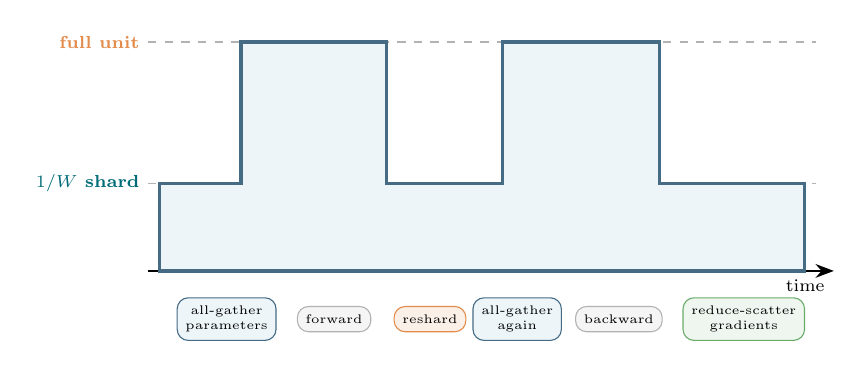
\begin{tikzpicture}[x=.82cm,y=.85cm,scale=.90,transform shape,every node/.style={font=\scriptsize}]
    \draw[-{Stealth},thick] (0,0)--(11.8,0) node[below left]{time};
    \draw[dashed,neutrallight] (0,3.8)--(11.5,3.8);
    \draw[dashed,neutrallight] (0,1.45)--(11.5,1.45);
    \node[left,font=\scriptsize\bfseries,text=warningdraw] at (0,3.8) {full unit};
    \node[left,font=\scriptsize\bfseries,text=accentdark] at (0,1.45) {$1/W$ shard};
    \fill[themebluebg,draw=themebluedraw,very thick]
      (.2,0)--(.2,1.45)--(1.6,1.45)--(1.6,3.8)--(4.1,3.8)--(4.1,1.45)--(6.1,1.45)--(6.1,3.8)--(8.8,3.8)--(8.8,1.45)--(11.3,1.45)--(11.3,0)--cycle;
    \node[draw=themebluedraw,fill=themebluebg,rounded corners,align=center,font=\tiny] at (1.35,-.8) {all-gather\\parameters};
    \node[draw=neutrallight,fill=neutralbg,rounded corners,font=\tiny] at (3.20,-.8) {forward};
    \node[draw=warningdraw,fill=warningbg,rounded corners,font=\tiny] at (4.85,-.8) {reshard};
    \node[draw=themebluedraw,fill=themebluebg,rounded corners,align=center,font=\tiny] at (6.35,-.8) {all-gather\\again};
    \node[draw=neutrallight,fill=neutralbg,rounded corners,font=\tiny] at (8.10,-.8) {backward};
    \node[draw=successdraw,fill=successbg,rounded corners,align=center,font=\tiny] at (10.25,-.8) {reduce-scatter\\gradients};
  \end{tikzpicture}
  \par\vspace{2pt}
  \footnotesize Full parameters are transient around compute; the local shard is persistent.\par
\end{frame}

\section{Execution and wrapping}

\begin{frame}{One FSDP unit is a materialization boundary}
  \begin{columns}[t]
    \begin{column}{0.47\linewidth}
      \begin{block}{Large unit}
        fewer collectives\\larger peak all-gather\\less opportunity for overlap\\coarser memory release
      \end{block}
    \end{column}
    \begin{column}{0.47\linewidth}
      \begin{alertblock}{Tiny units}
        low peak materialization\\many latency-dominated collectives\\more metadata and scheduling overhead
      \end{alertblock}
    \end{column}
  \end{columns}
  \vfill
  Wrapping each Transformer block is a common starting point because it aligns materialization with a natural compute unit.
\end{frame}

\begin{frame}{Communication volume and exposure are different}
  \begin{itemize}
    \setlength{\itemsep}{8pt}
    \item \textbf{Volume}: total bytes transferred by all-gathers and reduce-scatters.
    \item \textbf{Exposure}: communication time that remains visible after overlap with compute.
    \item \textbf{Frequency}: number of collectives and their message sizes.
  \end{itemize}
  \begin{alertblock}{Why this matters}
    Two wrapping policies can move similar bytes but have very different step times because one creates many small latency-bound collectives or a longer exposed tail.
  \end{alertblock}
\end{frame}

\begin{frame}{Prefetching tries to move the next unit early}
  \begin{center}
  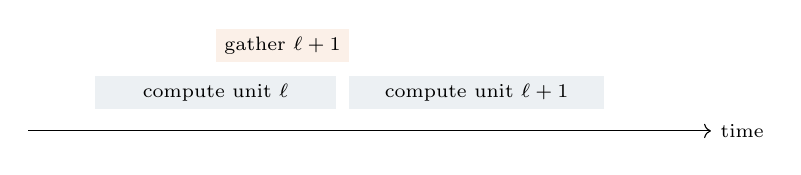
\begin{tikzpicture}[x=.85cm,y=.7cm,every node/.style={font=\scriptsize}]
    \draw[->] (0,0)--(10.2,0) node[right]{time};
    \fill[themebluecard] (1,.4) rectangle (4.6,1.0);
    \node at (2.8,.7) {compute unit $\ell$};
    \fill[warningbg] (2.8,1.25) rectangle (4.8,1.85);
    \node at (3.8,1.55) {gather $\ell+1$};
    \fill[themebluecard] (4.8,.4) rectangle (8.6,1.0);
    \node at (6.7,.7) {compute unit $\ell+1$};
  \end{tikzpicture}
  \end{center}
  \begin{alertblock}{Constraint}
    Prefetching improves overlap but raises transient memory because current and next full units may coexist.
  \end{alertblock}
\end{frame}

\begin{frame}{FSDP does not shard activation memory automatically}
  \begin{columns}[c]
    \begin{column}{0.50\linewidth}
      Full sharding reduces persistent parameter, gradient, and optimizer-state redundancy.
    \end{column}
    \begin{column}{0.46\linewidth}
      \begin{alertblock}{Still scales with batch and sequence}
        saved activations\\attention workspaces\\temporary full parameters\\communication buffers
      \end{alertblock}
    \end{column}
  \end{columns}
  \vfill
  Combine FSDP with activation checkpointing when activations, not model state, dominate the peak.
\end{frame}

\begin{frame}{Mixed precision has three separate decisions}
  \small
  \begin{tabular}{@{}>{\raggedright\arraybackslash}p{.30\linewidth}>{\raggedright\arraybackslash}p{.22\linewidth}>{\raggedright\arraybackslash}p{.38\linewidth}@{}}
    \toprule
    Quantity & Common choice & Main trade-off \\
    \midrule
    parameter compute dtype & BF16 & speed and temporary memory \\
    gradient reduction dtype & BF16 or FP32 & bandwidth versus numerical range \\
    optimizer state dtype & FP32 & stable moments at persistent cost \\
    \bottomrule
  \end{tabular}
  \vfill
  \begin{block}{Experimental rule}
    When comparing DDP and FSDP, align precision policy. Otherwise, memory and numerical differences have multiple causes.
  \end{block}
\end{frame}

\checkpoint{wrapping policy}
  {A run fits in memory but launches hundreds of tiny all-gathers and scales poorly. What wrapping change would you test, and which memory and timing quantities could regress?}

\section{Checkpointing and fair comparison}

\begin{frame}{A distributed checkpoint is a data layout}
  \begin{columns}[t]
    \begin{column}{0.31\linewidth}
      \begin{block}{Full}
        easy to consume\\expensive to gather\\rank 0 memory pressure
      \end{block}
    \end{column}
    \begin{column}{0.31\linewidth}
      \begin{block}{Sharded}
        scalable writes\\world-size coupling unless resharded
      \end{block}
    \end{column}
    \begin{column}{0.31\linewidth}
      \begin{block}{Distributed format}
        parallel I/O\\metadata and recovery complexity
      \end{block}
    \end{column}
  \end{columns}
  \begin{alertblock}{Completion protocol}
    Publish a checkpoint only after every shard and its metadata are durable. A directory that exists is not proof of a complete save.
  \end{alertblock}
\end{frame}

\begin{frame}{Checkpoint cadence and expected overhead}
  \begin{columns}[c]
    \begin{column}{0.68\linewidth}
      \centering
      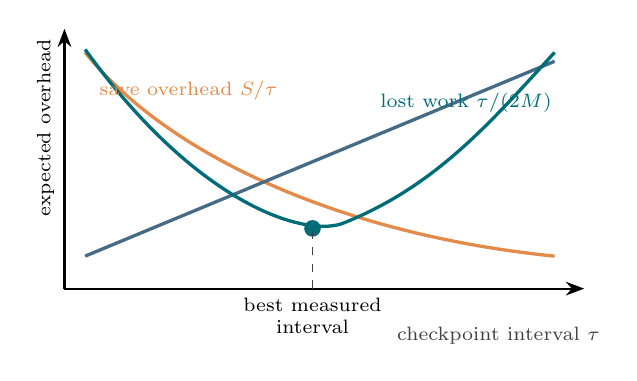
\begin{tikzpicture}[x=.75cm,y=.75cm,every node/.style={font=\scriptsize}]
        \draw[-{Stealth},thick] (0,0)--(8.8,0);
        \draw[-{Stealth},thick] (0,0)--(0,4.4) node[above,rotate=90,anchor=south east]{expected overhead};
        \draw[very thick,warningdraw] (.35,4.0) .. controls (1.8,2.2) and (4.8,.9) .. (8.3,.55);
        \draw[very thick,themebluedraw] (.35,.55)--(8.3,3.85);
        \draw[very thick,accentdark] (.35,4.05) .. controls (2.3,1.35) and (4.15,.85) .. (4.75,1.12) .. controls (6.3,1.75) and (7.2,2.8) .. (8.3,4.0);
        \fill[accentdark] (4.2,1.02) circle (3pt);
        \draw[dashed,neutraldark] (4.2,0)--(4.2,1.02);
        \node[text=warningdraw] at (2.1,3.35) {save overhead $S/\tau$};
        \node[text=accentdark] at (6.8,3.15) {lost work $\tau/(2M)$};
        \node[below,align=center] at (4.2,0) {best measured\\interval};
        \node[below,text=neutraldark] at (7.35,-.48) {checkpoint interval $\tau$};
      \end{tikzpicture}
    \end{column}
    \begin{column}{0.30\linewidth}
      \[
        \text{rate}\approx
        \frac{S}{\tau}+\frac{\tau}{2M}+\frac{L}{M}
      \]
      \small
      $M$: mean time between interruptions\\[4pt]
      $S$: exposed save time\\[4pt]
      $L$: recovery load time
    \end{column}
  \end{columns}
  \vspace{3pt}
  \footnotesize Measure durable save completion and restart time; file creation alone does not define $S$ or $L$.
  \smallsource{MVA Training and Deploying Large-Scale Models, Lecture 4 (2026)}
\end{frame}

\begin{frame}{A DDP--FSDP comparison needs a fixed contract}
  Match model, global token batch, optimizer, schedule, precision, data order, checkpoint cadence, and evaluation.
  \vspace{7pt}
  \begin{columns}[t]
    \begin{column}{0.47\linewidth}
      \begin{block}{Correctness evidence}
        first-update comparison\\loss trajectory\\resume equivalence
      \end{block}
    \end{column}
    \begin{column}{0.47\linewidth}
      \begin{block}{Systems evidence}
        peak allocated memory\\tokens per second\\collective exposure\\checkpoint time and size
      \end{block}
    \end{column}
  \end{columns}
\end{frame}

\begin{frame}{Choose FSDP when memory is the binding constraint}
  \begin{itemize}
    \setlength{\itemsep}{8pt}
    \item Prefer DDP when the model fits comfortably and communication simplicity wins.
    \item Prefer FSDP when replicated state blocks model size, batch size, or context.
    \item Tune wrapping and prefetch from traces, not from a universal recipe.
    \item Treat checkpoint load and resharding as part of the production design.
  \end{itemize}
\end{frame}

\checkpoint{memory prediction}
  {Estimate idealized model-state memory per rank for $P$ parameters, 16 bytes per parameter, and world size $W$. Then name three reasons the measured peak will be higher.}

\takeaways
  {ZeRO stages progressively shard optimizer state, gradients, and parameters.}
  {FSDP materializes one wrapped unit through all-gather and returns sharded gradients.}
  {Wrapping controls peak memory, collective size, frequency, and overlap.}
  {Checkpoint format and a matched DDP baseline are part of the system claim.}
\end{document}
